%\subsection{HW1}

%%%%%%%%%%%%% Q1

\par \noindent {We assume that households have log preferences ($\beta$), and the production
    technology satisfies
    \begin{eqnarray}
        Y_t = Z_t K_t^{\alpha}
    \end{eqnarray}
    with the parameters $ \alpha = 0.36,\ \beta = 0.99,\ \delta = 0.025$.
    The technology shock $Z$ follows a two-state Markov chain with transition matrix:
    \begin{eqnarray}
        \Pi = \begin{bmatrix}
            0.977 & 0.023 \\
            0.074 & 0.926
        \end{bmatrix}
    \end{eqnarray} and the two states of technology are $Z \in \left\{Z_g, Z_b\right\}$.
    The dynamic programming problem you are to solve is:
    \begin{eqnarray}
        \colorbox{black!10}{$ V(K,Z) = \max\limits_{K'} \; \log \left( ZK^{\alpha} + (1-\delta)K - K' \right) +
                \beta \E\left[ V(K',Z') \right] $}
    \end{eqnarray} where to save on notation any variable $X_t = X$ and $X_{t+1} = X'$.}

\begin{framedexercise}[VFI] Solve the stochastic dynamic programming problem via value function
    iteration over a discrete grid on $K$ of 1000 linearly spaced grid points
    over $[0.01, 90]$. Specifically, let $K_i \in \{0.01, 0.1001, \ldots, 90\}$.
    What are the differences in computing time between the un-parallelized versus
    parallelized versions for both deterministic and stochastic cases?
\end{framedexercise}

\begin{solution}
    I got the parallelized versions ran \textit{slower} than the un-parallelized versions
    in both deterministic and stochastic cases.
    My guess is that the model is too simple in a way that parallelization
    introduces an overhead issue.
\end{solution}

%%%%%%%%%%%%% Q2
\begin{framedexercise}[Value Function]Plot the value function over $K$ for each state $Z$.
    Is it \textit{increasing} (i.e. is $V(K_{i+1},Z) \geq V(K_i,Z)$ for $K_{i+1} > K_i$)?
    Is it \textit{concave} (in the sense that $V(K_{i+1},Z) - V(K_i,Z)$ is decreasing)?
\end{framedexercise}


\begin{solution}
    In Figure \ref{fig:VFI_stochastic} below, we see that the value functions are
    increasing and concave in $K$ for both states of technology $Z$. \qed
    \begin{figure}[H]
        \centering
        \caption{Value Function}
        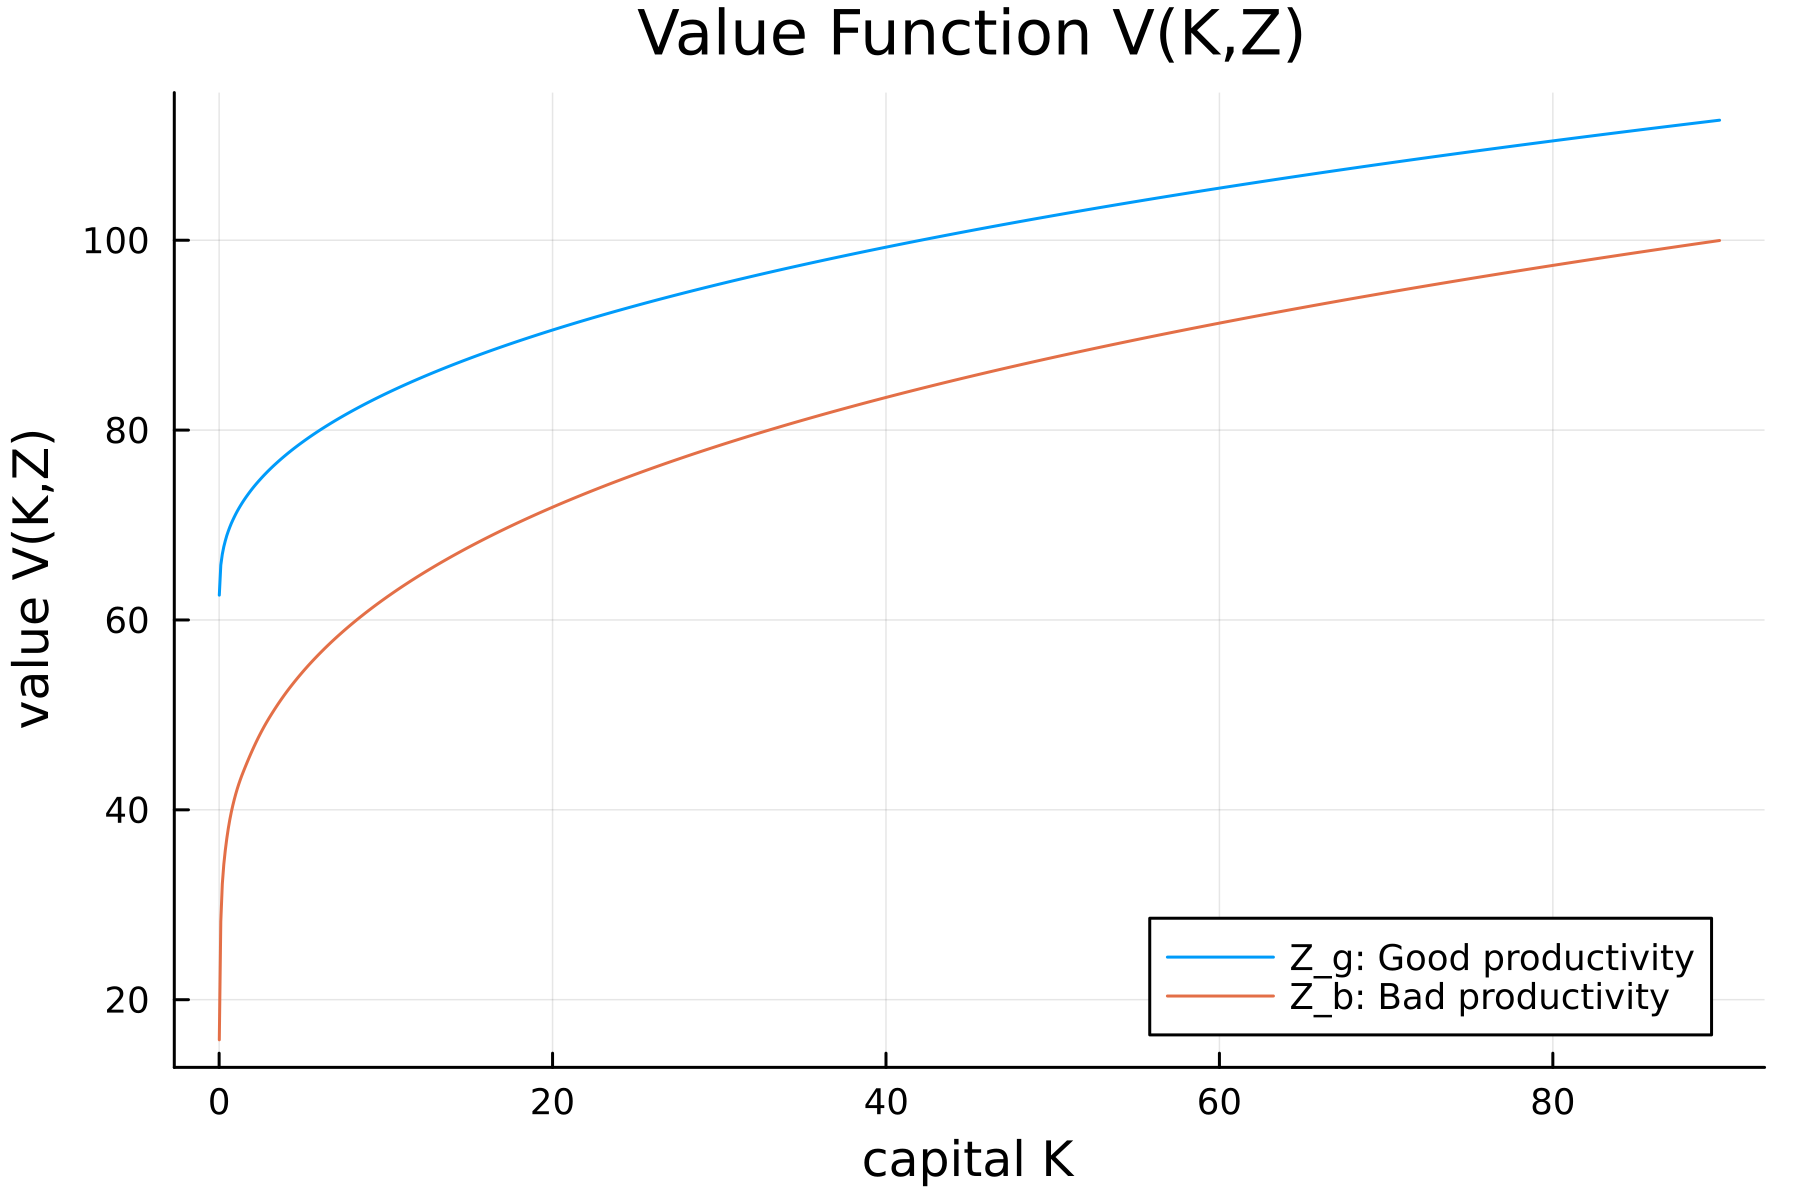
\includegraphics[width=0.55\textwidth, angle=0]
        {Parallel_Stochastic_Value_Functions.png}
        \label{fig:VFI_stochastic}
    \end{figure}
\end{solution}

% \newpage


%%%%%%%%%%%%% Q3(1)
\begin{framedexercise}[Decision Rule / Policy Function]
    Plot the decision rules $K'(K,Z)$ for each state $Z$ including a 45 degree line.
    Is the decision rule increasing/decreasing in $K$ and $Z$ (i.e. is
    $K'(K_{i+1},Z) \geq K'(K_i,Z)$ for $K_{i+1} > K_i$ and is $K'(K,Z_g) \geq K'(K,Z_b)$)?
\end{framedexercise}

\begin{solution} In Figure \ref{fig:Policy_stochastic} below, the decision rules are
    both increasing in capital level $K$ (positive slopes) and technology state $Z$ ($K'(K, Z_g)$
    lies above $K'(K, Z_b)$). \qed
    \begin{figure}[H]
        \centering
        \caption{Policy Function}
        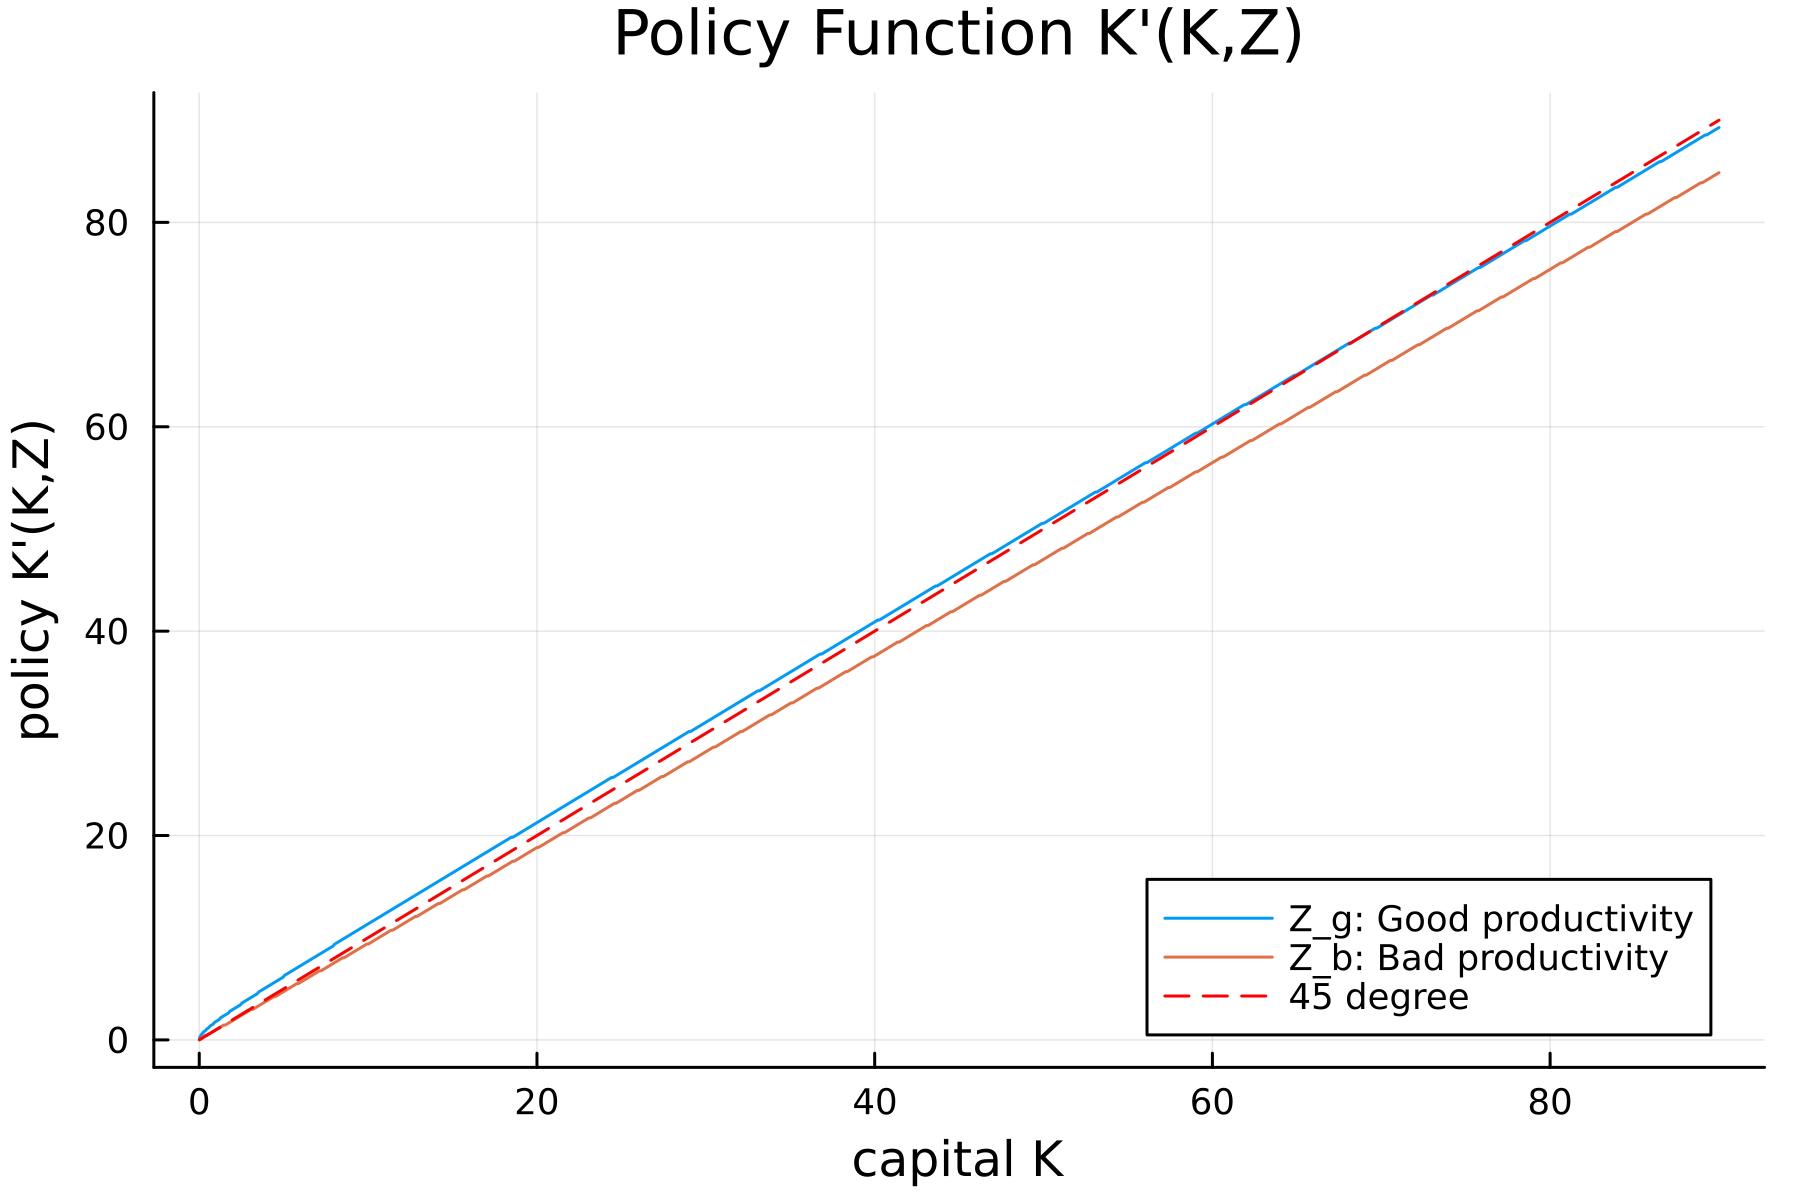
\includegraphics[width=0.55\textwidth, angle=0]
        {Parallel_Stochastic_Policy_Functions.png}
        \label{fig:Policy_stochastic}
    \end{figure}
\end{solution}

\newpage

%%%%%%%%%%%%% Q3(2)
\begin{framedexercise}[Saving / Policy Function Changes]
    Is saving increasing in $K$ and $Z$ (to see this, plot the change in the decision rule
    $K'(K,Z) - K$ across $K$ for each possible exogenous state $Z$)?
    Provide intuition in terms of the marginal benefit versus marginal cost
    of increasing capital holdings. What in the environment might lead to
    saving at low levels of capital and dissaving at high levels of capital?
\end{framedexercise}

\begin{solution} \par In Figure \ref{fig:Policy_changes_stochastic}, we notice that the saving schedule
    increases at lower levels of capital but then decreases at higher levels of capital
    if producer starts with good productivity.
    While in the opposite case where the producer starts with bad productivity,
    the producer always borrows (i.e., dissaving) for all levels of capital.

    \begin{figure}[H]
        \centering
        \caption{Policy Function Changes}
        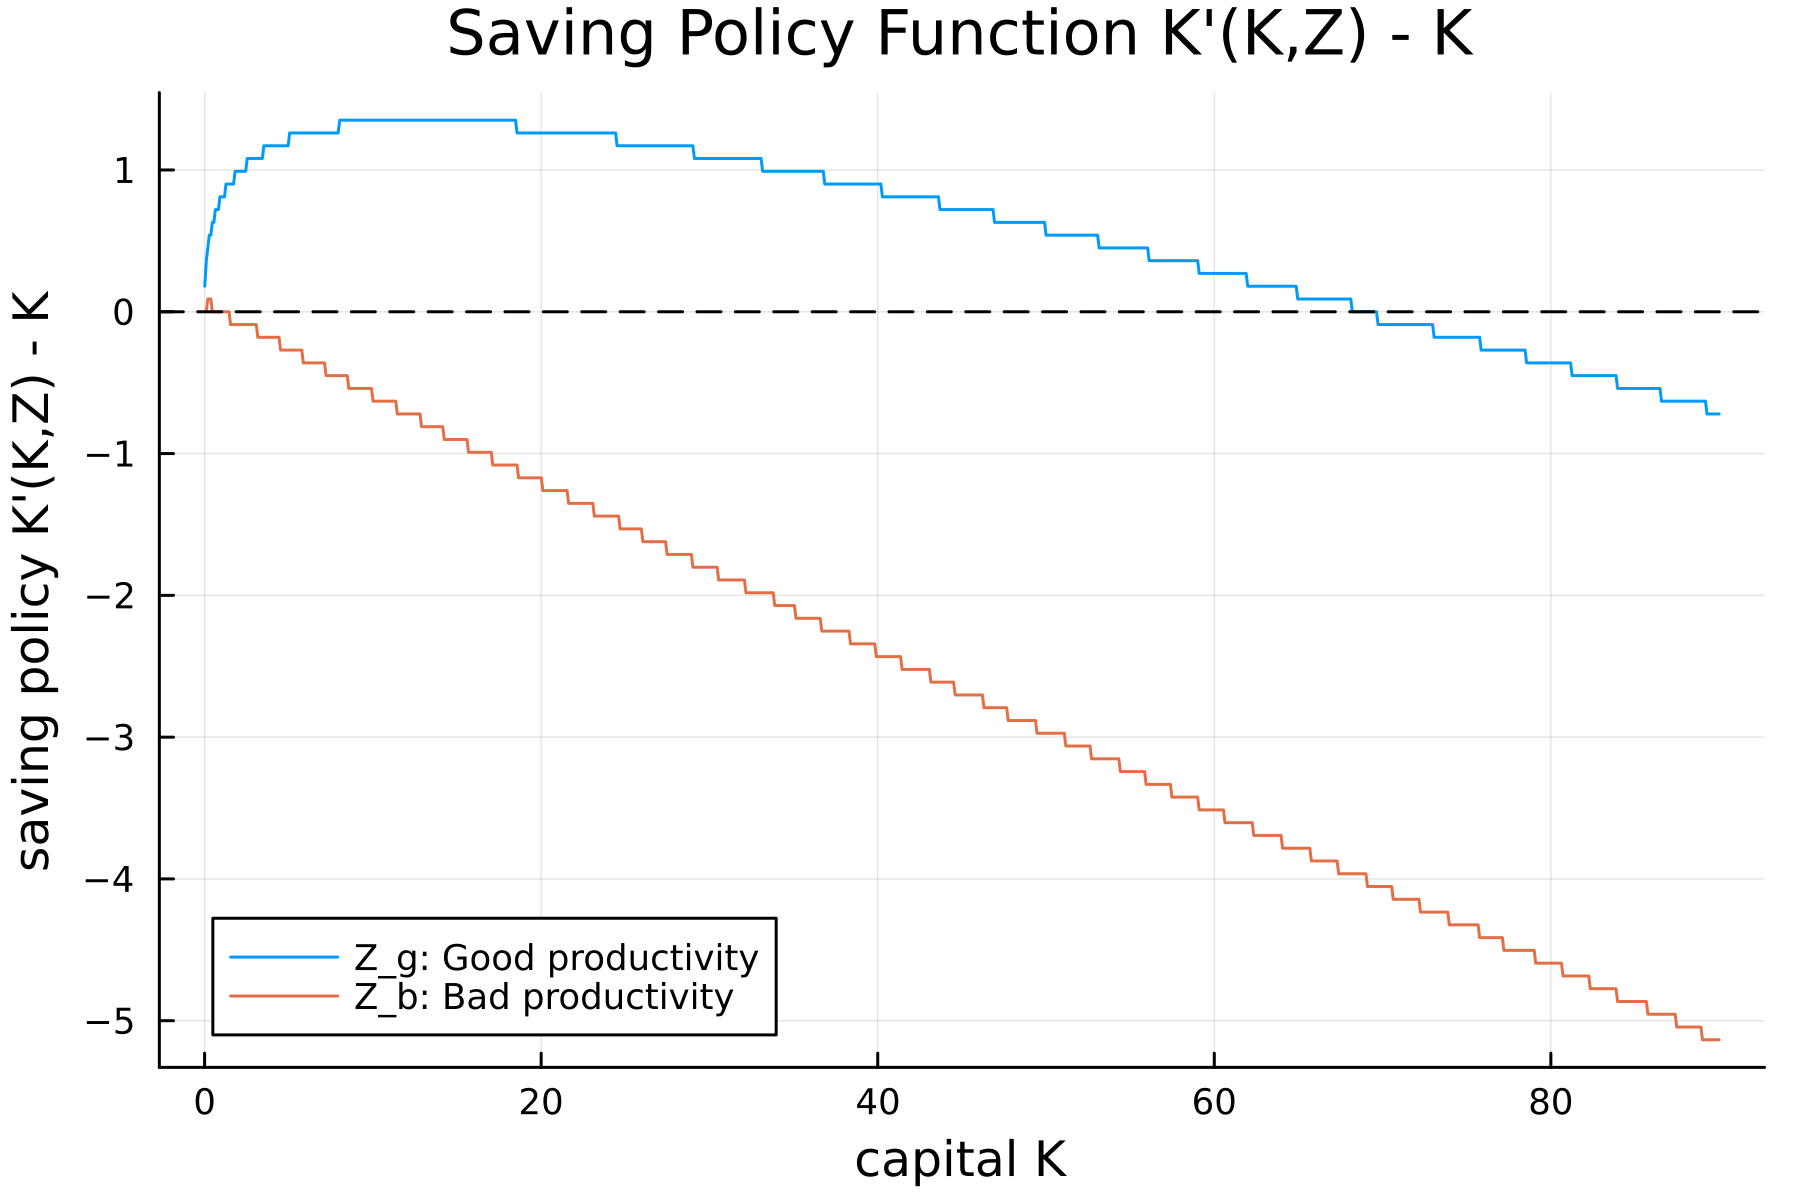
\includegraphics[width=0.55\textwidth, angle=0]
        {Parallel_Stochastic_Policy_Functions_Changes.png}
        \label{fig:Policy_changes_stochastic}
    \end{figure}

    \par In our DP formulation, the consumption is given by $C = ZK^{\alpha} + (1-\delta)K - K'$.
    With log utility, the consumption–saving decision should be shaped by:
    \begin{eqnarray}
        \underbrace{\frac{1}{C}}_{\text{\scriptsize MC of $\nearrow K$}} =
        \underbrace{\beta \E_{Z'}\left[ \frac{1}{C'}\left({\color{red} \alpha Z' (K')^{\alpha-1}} + (1 - \delta) \right) \right]}_{\text{\scriptsize MB of $\nearrow K$}},
    \end{eqnarray}
    \par \noindent \circled{1} For producer that starts with good productivity ($Z_g$),
    the transition matrix suggests that she is more likely to stay in good state,
    and the MB of increasing capital is high at low levels of capital
    (should $\searrow C$ for $\nearrow K$; saving). Then, as levels of capital increases, the MB diminishes so that
    she starts to dissave (should $\searrow K$ for $\nearrow C$; dissaving). \\[6pt]
    \par \noindent \circled{2} For producer that starts with bad productivity ($Z_b$), the transition matrix suggests that
    she is more likely to stay in bad state, and in that case the MB of increasing capital would be
    lower in every period due to $Z_b < 1$. Then there is no saving motive at all levels of capital.
\end{solution}